\documentclass[supercite]{Experimental_Report}

\title{~~~~~~数据结构实验~~~~~~}
\author{宁毓伟}
\school{计算机科学与技术学院}
\classnum{CS2101}
\stunum{U202115325}
\instructor{李剑军}
\date{2022年4月14日}

\usepackage{algorithm, multirow}
\usepackage{algpseudocode}
\usepackage{amsmath}
\usepackage{amsthm}
\usepackage{framed}
\usepackage{mathtools}
\usepackage{subcaption}
\usepackage{xltxtra} 
\usepackage{bm}
\usepackage{tikz}
\usepackage{tikzscale}
\usepackage{pgfplots}
\usepackage{xcolor}
\usepackage{listings}
\usepackage{float}
\usepackage{graphicx}

\pgfplotsset{compat=1.16}

\newcommand{\cfig}[3]{
  \begin{figure}%[htb]
    \centering
    \includegraphics[width=#2\textwidth]{images/#1.tikz}
    \caption{#3}
    \label{fig:#1}
  \end{figure}
}

\newcommand{\sfig}[3]{
  \begin{subfigure}[b]{#2\textwidth}
    \includegraphics[width=\textwidth]{images/#1.tikz}
    \caption{#3}
    \label{fig:#1}
  \end{subfigure}
}

\newcommand{\xfig}[3]{
  \begin{figure}%[htb]
    \centering
    #3
    \caption{#2}
    \label{fig:#1}
  \end{figure}
}

\newcommand{\rfig}[1]{\autoref{fig:#1}}
\newcommand{\ralg}[1]{\autoref{alg:#1}}
\newcommand{\rthm}[1]{\autoref{thm:#1}}
\newcommand{\rlem}[1]{\autoref{lem:#1}}
\newcommand{\reqn}[1]{\autoref{eqn:#1}}
\newcommand{\rtbl}[1]{\autoref{tbl:#1}}

\algnewcommand\Null{\textsc{null }}
\algnewcommand\algorithmicinput{\textbf{Input:}}
\algnewcommand\Input{\item[\algorithmicinput]}
\algnewcommand\algorithmicoutput{\textbf{Output:}}
\algnewcommand\Output{\item[\algorithmicoutput]}
\algnewcommand\algorithmicbreak{\textbf{break}}
\algnewcommand\Break{\algorithmicbreak}
\algnewcommand\algorithmiccontinue{\textbf{continue}}
\algnewcommand\Continue{\algorithmiccontinue}
\algnewcommand{\LeftCom}[1]{\State $\triangleright$ #1}

\newtheorem{thm}{定理}[section]
\newtheorem{lem}{引理}[section]

\colorlet{shadecolor}{black!15}

\theoremstyle{definition}
\newtheorem{alg}{算法}[section]

\def\thmautorefname~#1\null{定理~#1~\null}
\def\lemautorefname~#1\null{引理~#1~\null}
\def\algautorefname~#1\null{算法~#1~\null}

%代码插入设置

\lstset{breaklines}  					%让LaTeX自动将长的代码行换行排版
\lstset{extendedchars=false}   			%这一条命令可以解决代码跨页时,章节标题,页眉等汉字不显示的问题
\lstset{language=C++, 					%用于设置语言为C++
    identifierstyle=,
    basicstyle=\ttfamily,
    stringstyle=\ttfamily,
    showstringspaces=false,
    frame=shadowbox, 					%边框
    captionpos=b
}

\begin{document}

\lstset{language=C++}
\lstset{
	basicstyle          =   \sffamily,          % 基本代码风格
	keywordstyle        =   \bfseries,          % 关键字风格
	commentstyle        =   \rmfamily\itshape,  % 注释的风格,斜体
	stringstyle         =   \ttfamily,  % 字符串风格
	flexiblecolumns,                % 别问为什么,加上这个
	numbers             =   left,   % 行号的位置在左边
	showspaces          =   false,  % 是否显示空格,显示了有点乱,所以不现实了
	numberstyle         =   \zihao{-5}\ttfamily,    % 行号的样式,小五号,tt等宽字体
	showstringspaces    =   false,
	captionpos          =   t,      % 这段代码的名字所呈现的位置,t指的是top上面
	%frame               =   lrtb,   % 显示边框
}

\maketitle
\clearpage
\pagenumbering{Roman}

\tableofcontents[level=2]
\clearpage
\pagenumbering{arabic}



\section{基于链式存储结构的线性表实现}

所谓基于链式存储结构的线性表其实就是我们常说的链表。当然,再继续细分下去还有链式栈,链式队列这么些分法。下面的实验中主要涉及对于链表的数据类型,数据之间的关系以及基本操作及其实现方式等内容。

\subsection{问题描述}
线性表在物理内存中可以以链表表的方式实现,即物理上存储位置不一定相邻的两个元素通过指针连结,成为线性表中的相邻元素,且数据元素的前后关系不变。

\subsubsection{实验目的}
\begin{enumerate}
	\item 加深对链表的概念、基本运算的理解;
	\item 熟练掌握链表的逻辑结构与物理结构的关系;
	\item 以链表作为物理结构,熟练掌握链式线性表基本运算的实现。
\end{enumerate}

\subsubsection{数据类型}
链表元素的数据类型(ElemType)应该由链表的使用者进行定义,但为了便于描述链表的功能,笔者将在下文中假定链表的数据元素类型为整型(int)。

\subsubsection{元素关系}
链表中的元素之间的关系是前驱和后继的有序关系,在链表的定义过程中将会体现这一点。

\subsubsection{基本操作}
对于链表而言,最重要的部分是其基本操作,下面是待实现的基本操作:

\begin{description}
	\item[基本功能] (1)初始化表:函数名称是InitList(L);初始条件是线性表L不存在;操作结果是构造一个空的线性表;
	\item[基本功能] (2)销毁表:函数名称是DestroyList(L);初始条件是线性表L已存在;操作结果是销毁线性表L;
	\item[基本功能] (3)清空表:函数名称是ClearList(L);初始条件是线性表L已存在;操作结果是将L重置为空表;
	\item[基本功能] (4)判定空表:函数名称是ListEmpty(L);初始条件是线性表L已存在;操作结果是若L为空表则返回TRUE,否则返回FALSE;
	\item[基本功能] (5)求表长:函数名称是ListLength(L);初始条件是线性表已存在;操作结果是返回L中数据元素的个数;
	\item[基本功能] (6)获得元素:函数名称是GetElem(L,i,e);初始条件是线性表已存在,1≤i≤ListLength(L);操作结果是用e返回L中第i个数据元素的值;
	\item[基本功能] (7)查找元素:函数名称是LocateElem(L,e,compare());初始条件是线性表已存在;操作结果是返回L中第1个与e满足关系compare()关系的数据元素的位序,若这样的数据元素不存在,则返回值为0;
	\item[基本功能] (8)获得前驱:函数名称是PriorElem(L,cur,pre);初始条件是线性表L已存在;操作结果是若cur是L的数据元素,且不是第一个,则用pre返回它的前驱,否则操作失败,pre无定义;
	\item[基本功能] (9)获得后继:函数名称是NextElem(L,cur,next);初始条件是线性表L已存在;操作结果是若cur是L的数据元素,且不是最后一个,则用next返回它的后继,否则操作失败,next无定义;
	\item[基本功能] (10)插入元素:函数名称是ListInsert(L,i,e);初始条件是线性表L已存在,1≤i≤ListLength(L)+1;操作结果是在L的第i个位置之前插入新的数据元素e。
	\item[基本功能] (11)删除元素:函数名称是ListDelete(L,i,e);初始条件是线性表L已存在且非空,1≤i≤ListLength(L);操作结果:删除L的第i个数据元素,用e返回其值;
	\item[基本功能] (12)遍历表:函数名称是ListTraverse(L),初始条件是线性表L已存在;操作结果是依次对L的每个数据元素输出打印到屏幕上。\\ 
	\item[附加功能] (1)最大连续子数组和:函数名称是MaxSubArray(L); 初始条件是线性表L已存在且非空,请找出一个具有最大和的连续子数组(子数组最少包含一个元素),操作结果是其最大和;
	\item[附加功能] (2)和为K的子数组:函数名称是SubArrayNum(L,k); 初始条件是线性表L已存在且非空, 操作结果是该数组中和为k的连续子数组的个数;
	\item[附加功能] (3)顺序表排序:函数名称是sortList(L);初始条件是线性表L已存在;操作结果是将L由小到大排序;
	\item[附加功能] (4)实现线性表的文件形式保存:其中,需要设计文件数据记录格式,以高效保存线性表数据逻辑结构(D,{R})的完整信息;需要设计线性表文件保存和加载操作合理模式。
	\item[附加功能] (5)实现多个线性表管理:设计相应的数据结构管理多个线性表的查找、添加、移除等功能。
\end{description}


\subsection{系统设计}
本系统中首先定义了一些宏以及数据类型。宏定义用作状态的表示,如“成功状态”: OK ,“错误状态” : ERROR。

系统的线性表采用先进先出的链式存储结构。

系统有一个菜单供用户进行功能选择,用户可以根据提示信息通过键盘输入相应的字符来完成功能的选择。

在多线性表的定义中笔者利用一个数组(list)来保存多个线性表的结点,并用结点数组(listTail)来保存相应的结点,保存结点的目的是为了在对线性表进行元素追加的时候操作更为简便。
在系统中笔者维护一个整型变量nowIndex作为当前用户操作的线性表的下标,在用户每次更换操作对象时nowIndex的值也随之改变。这样一来就实现了多线性表的操作。

\subsection{系统实现}

\subsubsection{系统环境}
\begin{verbatim}
OS: Manjaro Linux x86_64(操作系统) 
Kernel: 5.15.32-1-MANJARO(内核)
CPU: AMD Ryzen 7 5800H with Radeon Graphics (16) 
Memory: 13898MiB
gcc version 11.2.0 (GCC)
\end{verbatim}
注意,若要在windows中运行本程序可以选择在WSL中运行或在window命令行中调用g++命令将cpp文件重新编译生成windows下的可执行文件(.exe)。



\subsubsection{宏定义以及数据类型定义}
\begin{verbatim}
#define TRUE 1              // 状态宏定义 
#define FALSE 0
#define OK 1
#define ERROR 0
#define INFEASIBLE -1
#define OVERFLOW -2
typedef int status;
typedef int ElemType;       //数据元素类型定义
#define LIST_INIT_SIZE 100  // 初始大小以及增量的宏定义
#define LISTINCREMENT  10
\end{verbatim}

\subsubsection{链结点类型}
系统的线性表采用先进先出的链式存储结构,为此我们需要对结点类型进行定义:
\begin{verbatim}
typedef struct LNode{       //单链表(链式结构)结点的定义
    ElemType data;
    struct LNode *next;
}LNode,*LinkList;
\end{verbatim}

\subsubsection{多线性表的实现方式}
多线性表定义如下:

其中的list数组用于保存各个链表的结点,listTail数组用于保存各个链表的结点。保存结点的目的是为了在对线性表进行元素追加的时候操作更为简便。
length表示该结构含有的链表个数,size表示该结构目前最多可以存放的链表个数。
\begin{verbatim}
typedef struct {      // 多链表定义!  
LinkList* list; LinkList* listTail;
int length; int size;
}Lists;
\end{verbatim}

\subsubsection{线性表基本操作的实现}
下面是线性表基本操作的实现原理,源代码位于附录B中。
\begin{enumerate}
	\item 链表的初始化InitList(L):\\这个函数的实现比较简单,先对传入的链表L进行判断,若L不存在
	      ,则可以进行初始化,为L动态分配一结点的空间作为结点并返回OK。
	      若L存在,初始化会使L中元素丢失,故不能将L初始化,此时应该返回INFEASIBLE(不可执行)。

	\item 链表的销毁DestroyList(L):\\首先判断链表是否存在,若不存在则不能够销毁,若链表存在
	      则对结点实施内存释放操作。内存释放过程如下:先用指针p指向结点,接着维护一个指针tmp使其
	      指向p的下一结点,接着将p指向的空间释放掉,再让p指向tmp所指向结点(即原来p的下一结点),
	      重复上述操作直到将L中的所结点都释放完,最后将L设置为NULL。
	
	\item 清空表ClearList(L):\\首先判断链表是否存在,如果不存在则不能够清空,返回INFEASIBLE(不可执行)。
	      若链表存在,则对结点实施内存释放操作。内存释放过程如下:先用指针p指向首元结点,接着维护一个指针tmp使其
	      指向p的下一结点,接着将p指向的空间释放掉,再让p指向tmp所指向结点(即原来p的下一结点),
	      重复上述操作直到将L中的所结点都释放完,最后将L的下一结点(L->next)设置为NULL。
	\item 判断空表ListEmpty(L):\\首先判断链表是否存在,如不存在则返回INFEASIBLE。若L存在,则判断L的下一结点(L->next)
	      是否为NULL,是则返回TRUE,不是则返回FALSE。

	\item 求表长ListLength(L):\\首先判断链表是否存在,如果不存在则不能够求表长,返回INFEASIBLE。
	      如果L存在,则令指针p指向L的结点,同时维护一个变量cnt(count的缩写),将其初始化为0,接着移动指针p,
	      每移动一次则cnt加1,当到L的最后一结点时不再移动,此时得到的cnt值就是链表的长度,将其返回即可。

	\item 获取元素GetElem(L,i,e):\\其中i是希望查找的元素的序号(从1开始计数),e是用于返回所找到的元素值。
	      第一步先判断表是否存在,若不存在,则返回INFEASIBLE。接着判断i的取值是否恰当,如果i的取值小于1
	      或大于链表的长度,则返回ERROR表示下标不存在。接下来就可以用p指向结点,让p向后移动,每次移动i同时减1,
	      当i减到0时p不再移动,此时p指向的便是目结点,将结点的数据域的值赋给e则可以返回OK。

	\item 查找元素LocateElem(L,e):\\查找元素e的下标:首先判断链表是否存在,如果不存在则不能够查找元素,返回INFEASIBLE。如果L存在,
	      则用指针p指向L的结点,同时维护一个变量index,将其初始化为0,接着移动指针p,p每移动一次,index的
	      值就加1,当p所结点的数据域取值和元素e的值相同,则将index返回,如果p指针移动到了L的尾部但仍没有
	      发现元素e,则返回ERROR表示没有找到该元素。

	\item 获取前驱PriorElem(L,e,pre):\\将e元素的前驱元素用pre返回: 首先判断链表是否存在,如果不存在则不能够查找前驱元素,返回INFEASIBLE。
	      如果L存在,则用p指向L的结点的下一结点,向后移动p,当p所结点的后结点的指针域的值与e相同,则将p所指结点的数据域的值赋给pre,并且返回OK。若p到达链表的结点还没有找到e,则返回ERROR表示找不到。

	\item 获取后继NextElem(L,e,next):\\将e元素的后继元素用next返回:首先判断链表是否存在,如果不存在则不能够查找后继元素,返回INFEASIBLE。
	      如果L存在,则用指针p指向L的首元结点,移动指针p,当p所结点的后结点的指针域的值与e相同时停止移动,此时判断p的下一结点是否存在,
	      存在则将其数据域的值赋给next并返回OK,不存在或没有找到元素e则返回ERROR表示找不到。

	\item 插入元素ListInsert(L,i,e):\\在位置i插入元素e:首先判断链表是否存在,如果不存在则不能够插入元素,返回INFEASIBLE。
	      接着判断i的取值是否恰当,如果i的取值小于1,则返回ERROR表示下标不存在。
	      接着先将i减1,令指针p指向结点并且移动p,每次移动i同时减1,当i减到0时p不再移动,此时先创建一个指针变量tmp,为该指针变量分配一结点的空间,
	      给tmp指向结点的数据域赋值为e,同时tm结点的下一结点设置为p的下一结点,而p的下一结点则设置为tmp,接着让L的长度(L.length)加一后返回OK。
	      若p到达链表的结点i还没有减到0,则返回ERROR表示下标不存在。

	\item 删除元素ListDelete(L,i,e)):\\在位置i删除元素e:首先判断链表是否存在,如果不存在则不能够删除元素,返回INFEASIBLE。
	      接着判断i的取值是否恰当,如果i的取值小于1,则返回ERROR表示下标不存在。
	      接着先将i减1,令指针p指向结点并且移动p,每次移动i同时减1,当i减到0时p不再移动,此时判断p的下一结点是否存在,如存在则先用一个临时指针tmp指向p的下一结点,并且将p的下结点设置为p的下一结点的下一结点(p->next = p->netx->next),接着将tm结点的数据域值赋给e并释放tmp所指的空间,接着让L的长度(L.length)减一后即可返回OK。
	      若p到达链表的结点i还没有减到0,或者i为0时p的下一结点为空,则返回ERROR表示下标不存在。

	\item 遍历表ListTraverse(L):\\按从头到尾的循序输出L中的元素:先对传入的链表L进行判断,如果L不存在则不能够遍历,返回INFEASIBLE。
	      如果L存在,则让指针p指向L的首元结点,接着移动指针p,每移动一次则将p所结点的数据域的值输出,直到p为空则不再移动并返回OK。
		  
	\item 链表反转reverseList(L):\\将链表中元素的循序反转:首先判断链表是否存在,如果不存在则不能够反转链表,返回INFEASIBLE。
	      如果链表的长度为0或为1,则直接返回OK,因为此时并不需要反转。
	      如果链表存在且长度大于1,则让指针p指向L的首元结点,指针nextOfp指向p的下一结点,接着用一个指针tmp记录nextOfp的下一结点,将nextOfp的下一结点设置为p(nextOfp->next = p),接着让将nextOfp的值赋给p,将tmp的值赋给nextOfp,重复上述操作直到将nextOfp的值为NULL后,将L的下一结点设置为p(L->next = p)后便可以返回OK。
	\item 删除链表中倒数第n结点RemoveNthFromEnd(L, n):先判断链表是否存在,如果不存在则不能够进行操作,返回INFEASIBLE。如果存在则创建一个变量index并将其初始化为L.length - n + 1,这就是给定n值的从正向数起的元素值,接着调用函数ListDelete()将序号为index的元素删除即可返回OK。

	\item 链表排序sortList(L):\\先判断链表是否存在,如果不存在则不能够进行排序,返回INFEASIBLE。如果存在则
	      将列表进行升序排序,先创建一个长度和链表长度一样的整型数组,接着将链表元素依次放到该数组中,对该数组进行快速排序,接着将数组中的元素值依次赋给链表中结点,完成后即可返回OK。

	\item 将链表数据保存在文件中saveList(L, FileName):\\先判断链表是否存在,如果不存在则不能够进行保存,返回INFEASIBLE。如果存在则将文件以二进制方打开,让指针p指向L的首元结点,将p所结点的数据域的值保存在文件中后将p移动到下一结点,重复上述操作直到p的值为NULL后即可返回OK。需要注意的是当打开文件后要判断文件是否打开成功,打开失败则应该返回ERROR表示文件未正常打开。

	\item 从文件中读取数据创建链表LoadList(L, FileName):先判断链表是否存在,如果链表存在且不为空则不能够进行创建,返回INFEASIBLE。如果链表不存在则为L动态分配一结点的空间,若链表存在且为空则不需要进行这一项操作,接着将文件以二进制的形式打开,接着创建一个tail指针指向L,再创建一个临时指针tmp,为tmp动态分配一结点的空间,从文件中读取一个数据到tmp中并且将tail所指的下一结点设置为tmp,最后将tmp的指针值赋给tail,重复上述操作直到文件指针移动到EOF处。
	      最后将tail所指的下一结点设置为NULL并返回OK。需要注意在打开文件时要判断打开是否成功,不成功则返回ERROR。
\end{enumerate}

\subsection{系统测试}
\subsubsection{菜单功能}
下面是菜单的截图:
\begin{figure}[htbp]
	\centering
	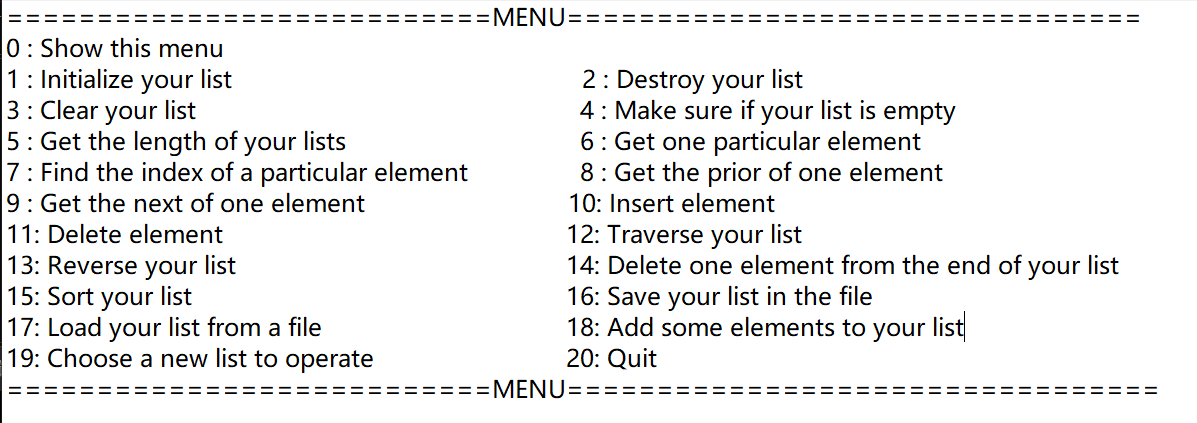
\includegraphics[scale = 0.7]{images/1.png}
	\caption{菜单}
\end{figure}

注意:以下各个函数测试时相互独立,进行各个功能测试初始数据与初始化链表并添加数据时的数据相同。

\subsubsection{初始化链表以及添加数据}
添加以下链表并初始化, 接着填入数据:

list1 : (空表)

list2 : 1, 2, 4, 6, 2

list3 : -10, 29, 8, 7

填入测试用例的操作以及截图如下:
操作:首先在命令行里面输入./LinkList.out以运行该程序,接着选择功能19添加一个名为listi(i = 1, 2, 3)的链表,选择功能1将其初始化后再选择功能18添加元素(i为1时不添加元素)。\newpage
\begin{figure}[htbp]
	\centering
	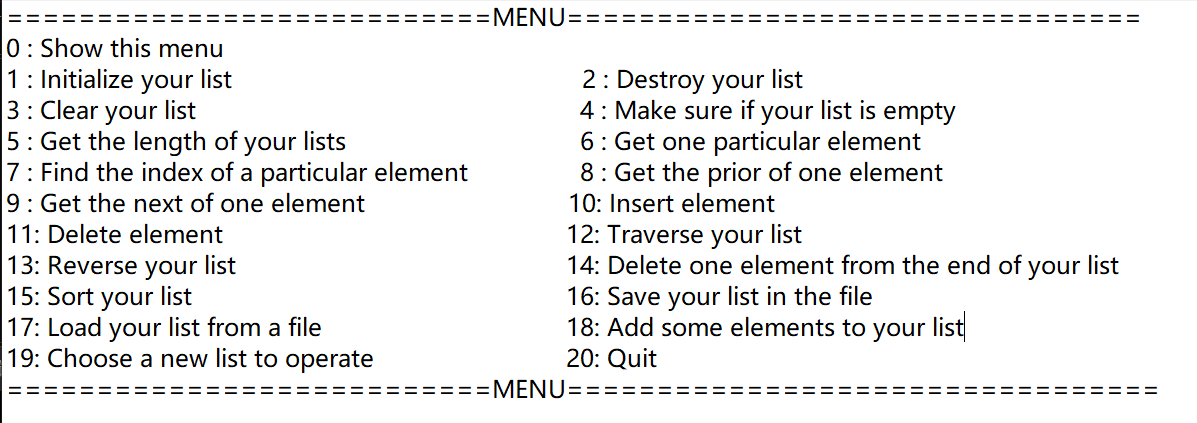
\includegraphics[scale = 0.7]{images/1.png}
	\caption{菜单}
\end{figure}

\subsubsection{销毁表}
先销毁list1(空表), 接着再次销毁list1。理论结果是第一次销毁成功,第二次销毁失败。实际结果如图所示:
\begin{figure}[htbp]
	\centering
	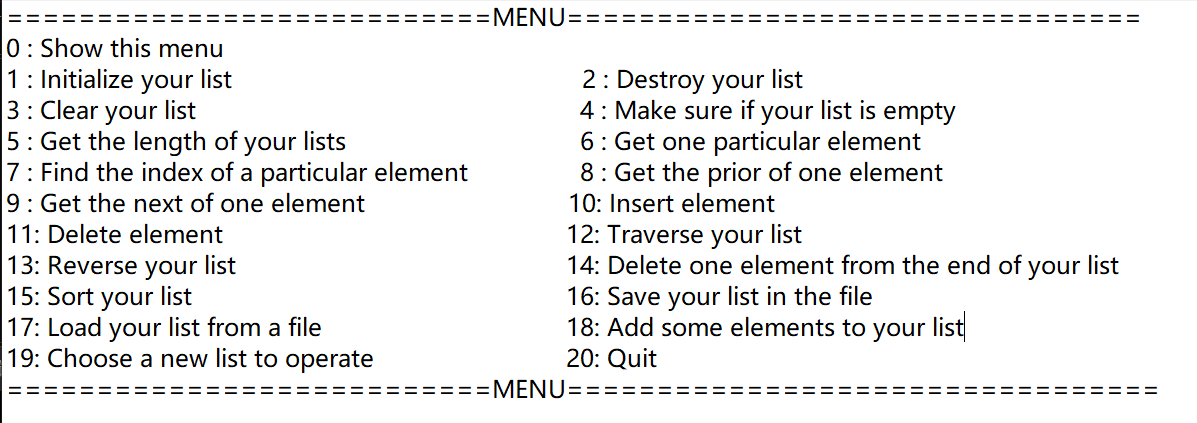
\includegraphics[scale = 0.7]{images/1.png}
	\caption{菜单}jie zhe
\end{figure}

\subsubsection{清空表}
首先对表list3进行清空,接着再次选择清空list3。理论结果是第一次清空成功,第二次清空失败。实际结果如截图所示:
\begin{figure}[htbp]
	\centering
	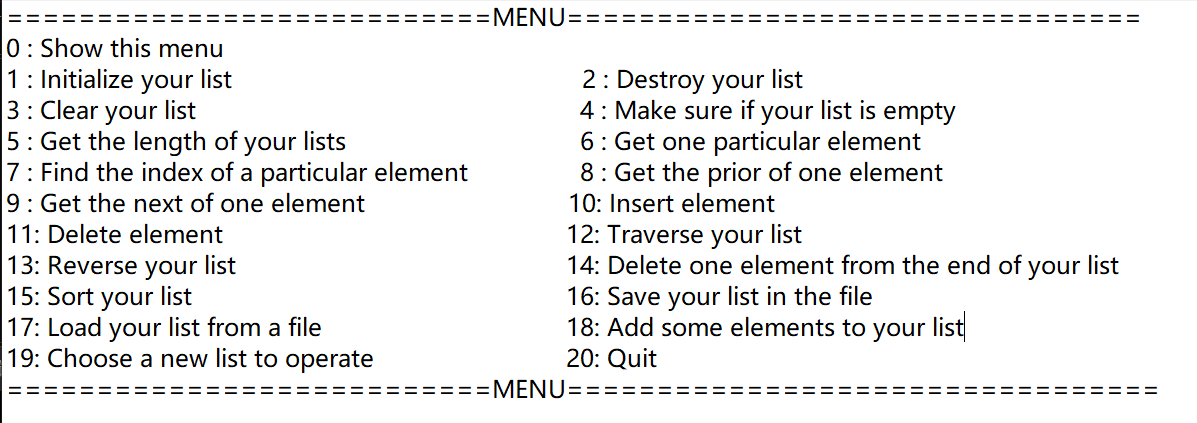
\includegraphics[scale = 0.7]{images/1.png}
	\caption{菜单}
\end{figure}
\subsubsection{判断空表}
选择对list2进行判断空表,接着对list1进行判断空表,理论结果是得到list2不为空,list1为空的信息。实际结果截图所示:
\begin{figure}[htbp]
	\centering
	%\vspace{}
	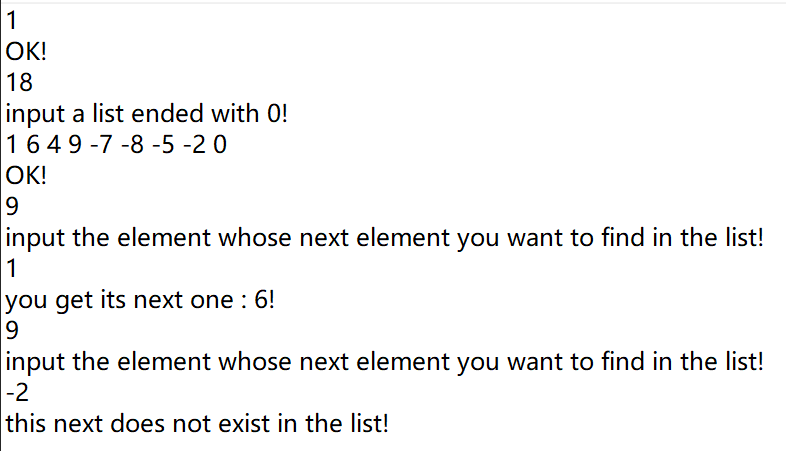
\includegraphics[scale = 0.7]{images/8.png}
	\caption{获取后继}
\end{figure}
\subsubsection{获取表长}
分别对list1, list2, list3求表长,理论结果是表长分别为0, 5, 4。实际结果如图所示:
\begin{figure}[htbp]
	\centering
	%\vspace{}
	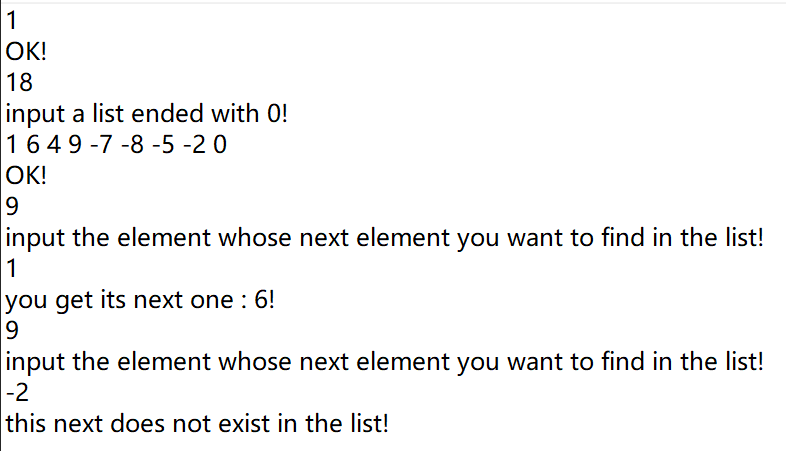
\includegraphics[scale = 0.7]{images/8.png}
	\caption{获取后继}
\end{figure}
\subsubsection{通过下标获取元素}
分别获取list2中下标为3以及下标为100的元素,理论结果是得到4以及下标不存在的信息。实际结果如图所示:
\begin{figure}[htbp]
	\centering
	%\vspace{}
	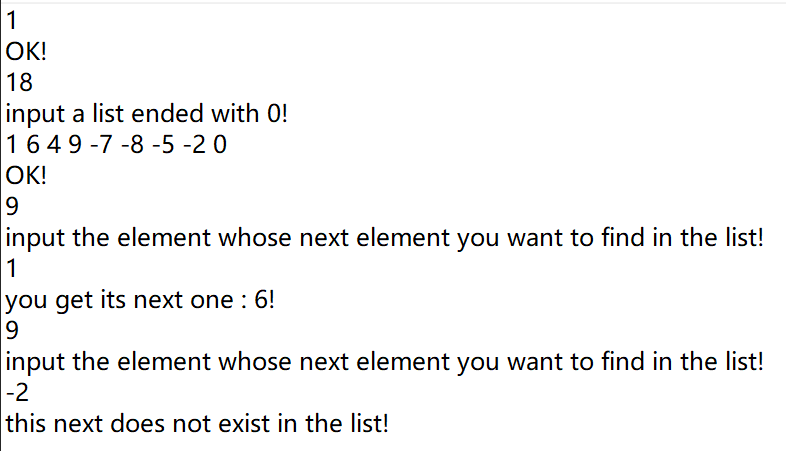
\includegraphics[scale = 0.7]{images/8.png}
	\caption{获取后继}
\end{figure}
\subsubsection{获取元素的下标}
获取list2中元素4的下标以及获取元素100的下标,理论结果是得到4的下标为3, 元素100不存在。实际结果如图所示:
\begin{figure}[htbp]
	\centering
	%\vspace{}
	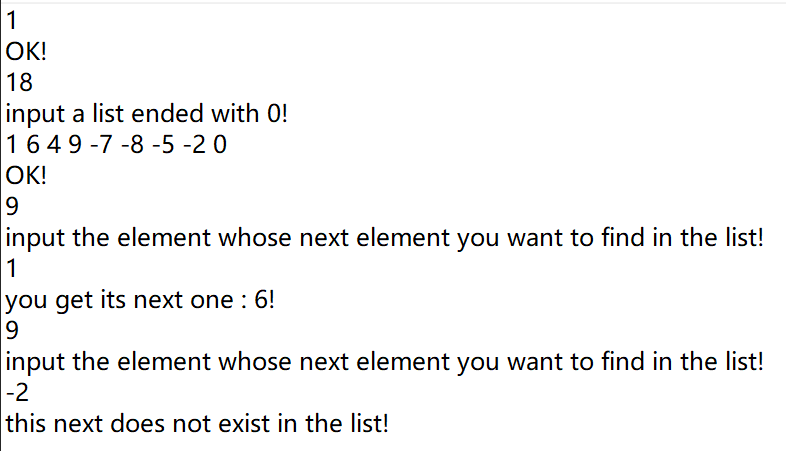
\includegraphics[scale = 0.7]{images/8.png}
	\caption{获取后继}
\end{figure}

\subsubsection{获取前驱}
分别获取list2中元素1, 2的前驱, 理论结果是1的前驱不存在, 2的前驱为1。实际结果如图所示:
\begin{figure}[htbp]
	\centering
	%\vspace{}
	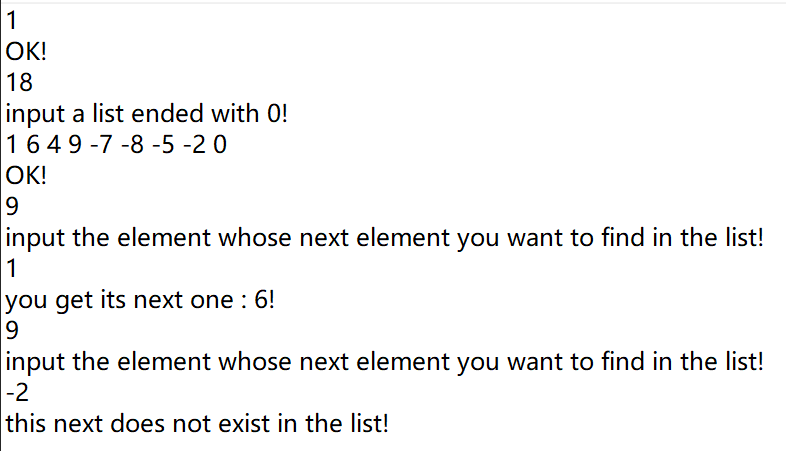
\includegraphics[scale = 0.7]{images/8.png}
	\caption{获取后继}
\end{figure}
%%%%%%%%%%%%%%%%%%%%%%%%%从此开始无图%%%%%%%%%%%%%%%%%%%%%%%%%%%%%%%%%%%%
\subsubsection{获取后继}
分别获取list3中元素8, 7的后继, 理论结果是8的后继是7, 7的后继不存在。实际结果如图所示:
\begin{figure}[htbp]
	\centering
	%\vspace{}
	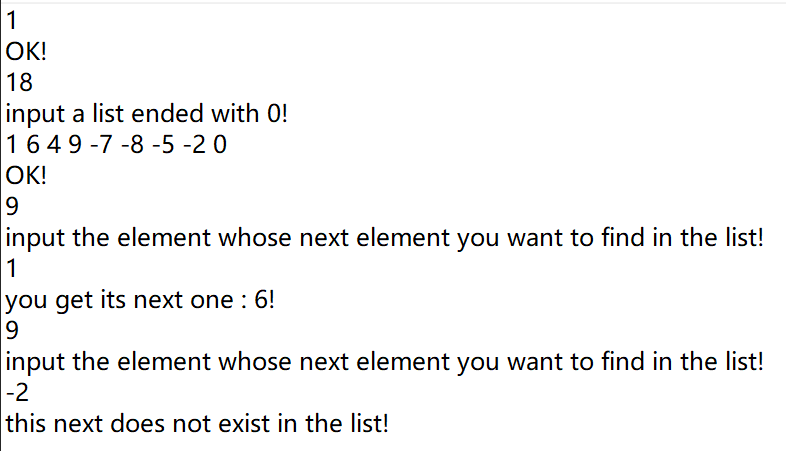
\includegraphics[scale = 0.7]{images/8.png}
	\caption{获取后继}
\end{figure}

\subsubsection{插入元素}
向list3中下标为2的位置插入元素10并接着向list3中下标为100的位置插入元素100,接着对表进行遍历,理论结果是第一次插入成功,第二次插入失败,并且遍历将得到\{-10, 10, 29, 8, 7\}。实际结果如下图所示:
\begin{figure}[htbp]
	\centering
	%\vspace{}
	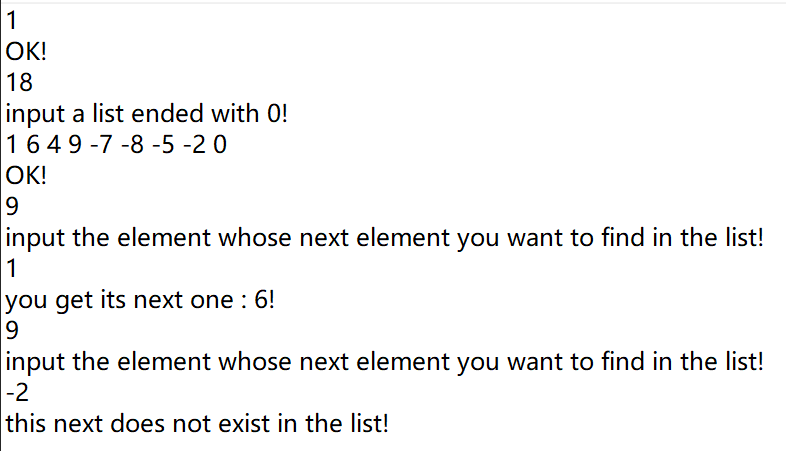
\includegraphics[scale = 0.7]{images/8.png}
	\caption{获取后继}
\end{figure}

\subsubsection{删除元素}
向list3中下标为2的位置删除元素10并接着向list3中下标为100的位置删除元素100,接着对表进行遍历,理论结果是第一次删除成功,第二次删除失败,并且遍历将得到\{-10, 29, 8, 7\}。实际结果如下图所示:
\begin{figure}[htbp]
	\centering
	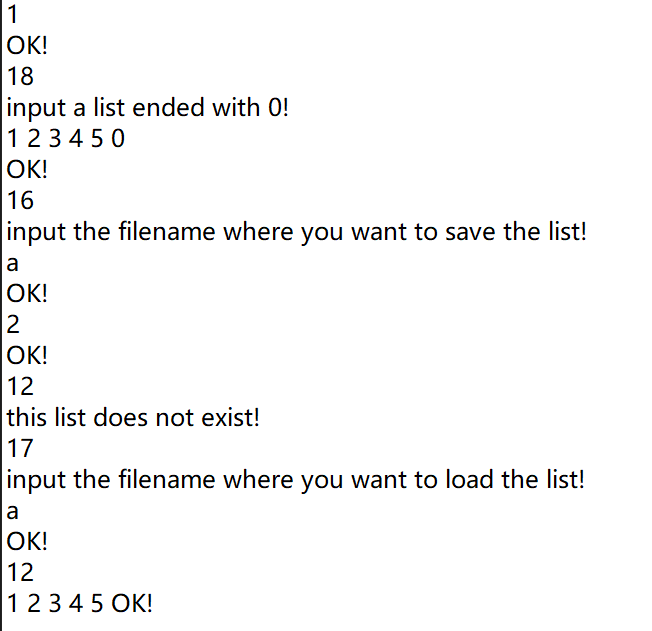
\includegraphics[scale = 0.8]{images/15.png}
	\caption{将链表保存在文件中以及从文件中读取链表}
\end{figure}

\subsubsection{遍历表}
分别对list1, list2, list3进行遍历, 理论结果是分别得到list1为空,list2 = \{1, 2, 4, 6, 2\}, list3 = \{-10, 29, 8, 7\}。实际结果如下图所示:
\begin{figure}[htbp]
	\centering
	%\vspace{}
	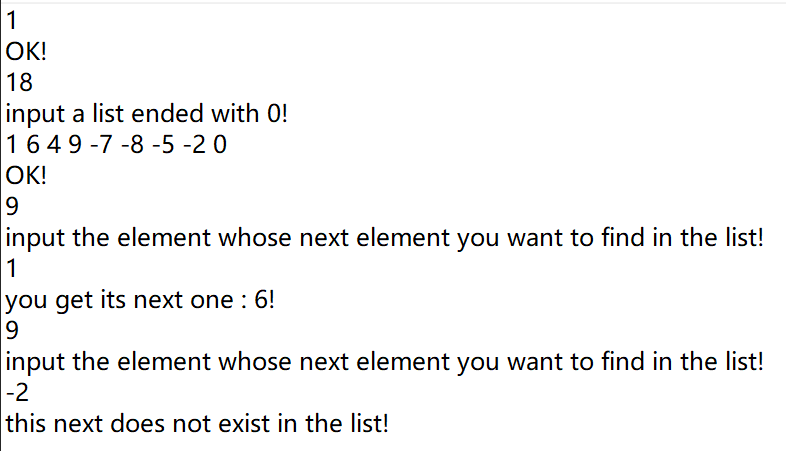
\includegraphics[scale = 0.7]{images/8.png}
	\caption{获取后继}
\end{figure}

\subsubsection{反转链表}
对list2进行反转后遍历, 理论结果得到\{2, 6, 4, 2, 1\}。实际结果如下图所示:
\begin{figure}[htbp]
	\centering
	%\vspace{}
	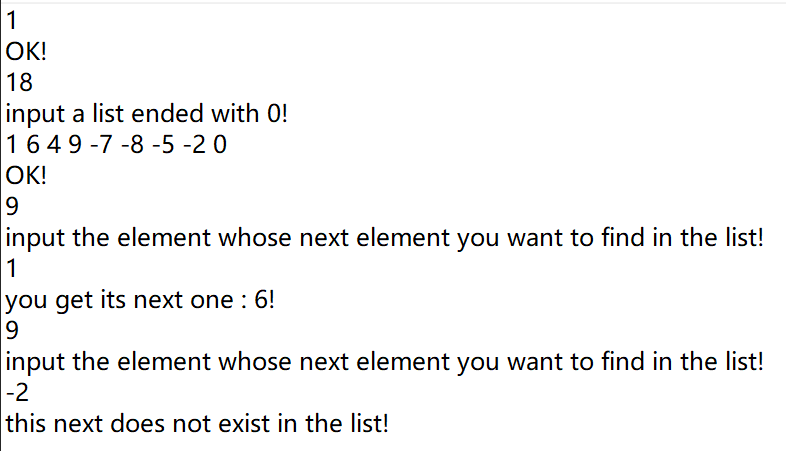
\includegraphics[scale = 0.7]{images/8.png}
	\caption{获取后继}
\end{figure}

\subsubsection{从尾部删除元素}
删除list2尾部第一个元素后进行遍历, 理论结果是得到\{1, 2, 4, 6\}。实际结果如下图所示:
\begin{figure}[htbp]
	\centering
	%\vspace{}
	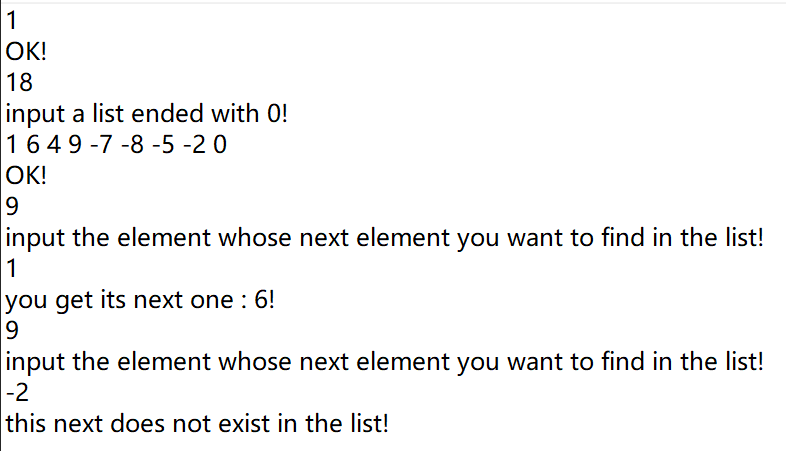
\includegraphics[scale = 0.7]{images/8.png}
	\caption{获取后继}
\end{figure}
\subsubsection{链表排序}
对list2排序后进行遍历, 理论结果是得到\{1, 2, 2, 4, 6\}。实际结果如下图所示:
\begin{figure}[htbp]
	\centering
	%\vspace{}
	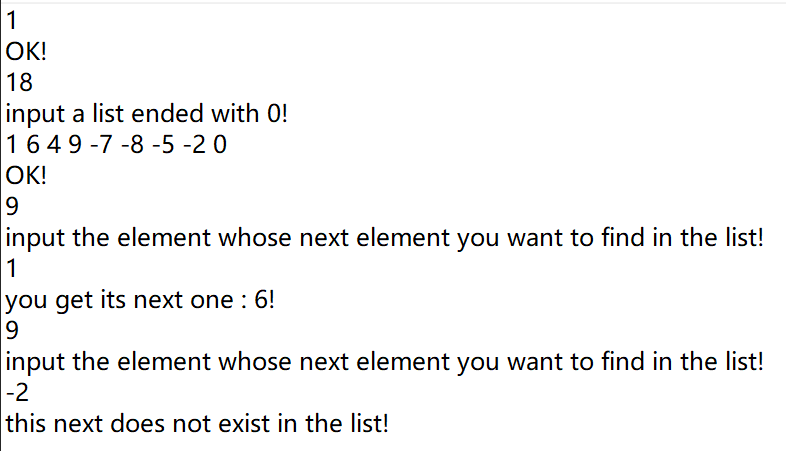
\includegraphics[scale = 0.7]{images/8.png}
	\caption{获取后继}
\end{figure}

\subsubsection{将链表保存在文件中后从文件中读取链表}
将list2保存在文件list中, 接着从list中读取链表到list1中,对list1进行遍历,理论结果是得到\{1, 2, 4, 6, 2\}。实际结果如下图所示:
\begin{figure}[htbp]
	\centering
	%\vspace{}
	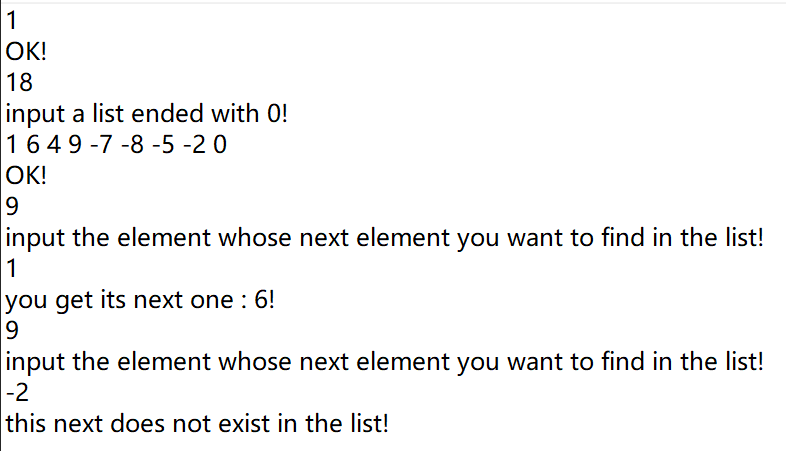
\includegraphics[scale = 0.7]{images/8.png}
	\caption{获取后继}
\end{figure}
\subsubsection{查找和删除链表}
查找名为list2的链表并将其删除,接着查找list2,理论结果是第一次得到list2的序号为2, 第二次查找失败。实际结果如下图所示:
\begin{figure}[htbp]
	\centering
	%\vspace{}
	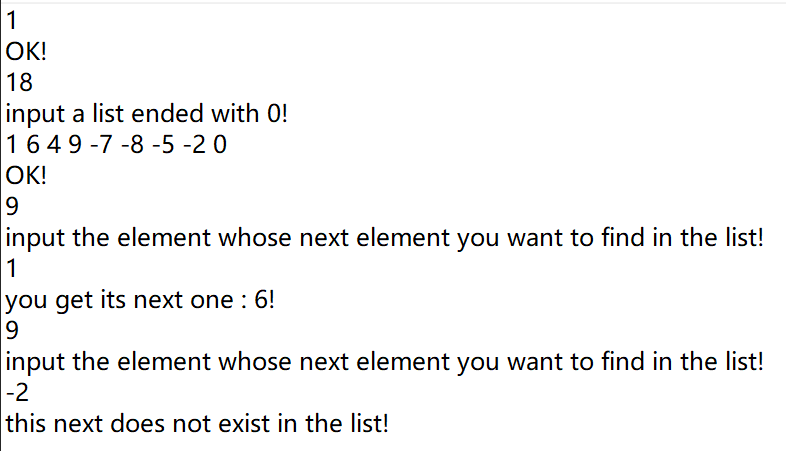
\includegraphics[scale = 0.7]{images/8.png}
	\caption{获取后继}
\end{figure}

\newpage
\subsection{实验小结}
\subsubsection{实验中遇到的问题及其解决方案}
第一次写链表时没有加入结点,导致自己无法分清楚清空链表和销毁链表的区别,经查阅资料后发现清空链表保留结点,而销毁链表不保留结点。解决方案:为每个链表加入一个结点后问题得到解决。

最开始时求表长功能返回的结果总是比正确结果要多1,笔者仔细查看代码后发现自己将表结点进行了一次计数,于是我将用于计数的指针p先指向首元结点后将问题解决。

由于笔者一开始没有安排插入一串元素的功能而只能一个个元素插入导致在进行测试时十分麻烦,于是我便为这个系统添加了一次性插入一串元素的功能让系统更加人性化。
\subsubsection{一些感悟}
基于链式存储结构的线性表实现的实验任务让我在学习完链表之后对链表的基本操作以及底层实现原理都更加的熟悉了
,实验过程中对于指针的移动操作让我对c语言的指针数据类型更加熟悉,在本次实验中我还增强了自己debug的能力,
对于断点调试等调试方法更加的熟练。同时,我还对{\LaTeX}这一排版工具进行了深入的了解,这些知识都将使我受益终身!
\newpage

\section{基于二叉链表的二叉树实现}
二叉树(Binary tree)是树形结构的一个重要类型。许多实际问题抽象出来的数据结构往往是二叉树形式,即使是一般的树也能简单地转换为二叉树,而且二叉树的存储结构及其算法都较为简单,因此二叉树显得特别重要。
\subsection{问题描述}

\subsubsection{实验目的}
\begin{enumerate}
	\item 加深对二叉树的概念、基本运算的理解;
	\item 熟练掌握二叉树的逻辑结构与物理结构的关系;
	\item 以二叉链表作为物理结构,熟练掌握二叉树基本运算的实现。
\end{enumerate}

\subsubsection{数据类型}
二叉树元素的数据类型是一个结构体类型,其中包含的三个部分分别是数据域,左孩子指针域以及右孩子指针域。其中数据域的类型 (ElemType) 应该由二叉树的使用者进行定义,但为了便于描述二叉树的功能,笔者将在下文中假定二叉树的数据域数据元素类型为整型 (int)。

\subsubsection{元素关系}
根据二叉结点类型的定义,每结点(称为结点)都有两个孩结点(孩结点可以为空),且孩结点有左孩结点以及有孩结点之分,故元素之间的关系可以有父子关系,兄弟关系。

\subsubsection{基本操作}
对于二叉树而言,最重要的部分就是二叉树的基本操作,下面是待实现的基本操作。
\begin{description}
	\item[基本功能] (1)创建二叉树:函数名称是CreateBiTree(T,definition);初始条件是definition 给出二叉树T的定义,根据带空子树的二叉树先序遍历序列definition构造一个二叉链表T(要求二叉树T中各结点关键字具有唯一性)。根指针指向根结点,不需要在根结点之上再增加头结点。输入序列为二叉树带空子树的先序遍历结点序列,每个结点对应一个整型的关键字和一个字符串,当关键字为0时,表示空子树,为-1表示输入结束
	\item[基本功能] (2)销毁二叉树:函数名称是DestroyBiTree(forest, int index);将森林forest中下标为index的二叉树销毁;
	\item[基本功能] (3)清空二叉树:函数名称是ClearBiTree (T);初始条件是二叉树T存在;操作结果是将二叉树T清空;
	\item[基本功能] (4)判定空二叉树:函数名称是BiTreeEmpty(forest,index);判断森林中下标为index的树是否为空,操作结果是若为空二叉树则返回TRUE,否则返回FALSE;
	\item[基本功能] (5)求二叉树深度:函数名称是BiTreeDepth(T);初始条件是二叉树T存在;操作结果是返回T的深度;
	\item[基本功能] (6)查找结点:函数名称是LocateNode(T,e);初始条件是二叉树T已存在,e是和T中结点关键字类型相同的给定值;操作结果是返回查找到的结点指针,如无关键字为e的结点,返回NULL;
	\item[基本功能] (7)结点赋值:函数名称是Assign(T,e,value);初始条件是二叉树T已存在,e是和T中结点关键字类型相同的给定值;操作结果是关键字为e的结点赋值为value;
	\item[基本功能] (8)获得兄弟结点:函数名称是GetSibling(T,e);初始条件是二叉树T存在,e是和T中结点关键字类型相同的给定值;操作结果是返回关键字为e的结点的(左或右)兄弟结点指针。若关键字为e的结点无兄弟,则返回NULL;
	\item[基本功能] (9)插入结点:函数名称是InsertNode(T,e,LR,c);初始条件是二叉树T存在,e是和T中结点关键字类型相同的给定值,LR为0或1,c是待插入结点;操作结果是根据LR为0或者1,插入结点c到T中,作为关键字为e的结点的左或右孩子结点,结点e的原有左子树或右子树则为结点c的右子树;特殊情况,c插入作为根结点?可以考虑LR为-1时,作为根结点插入,原根结点作为c的右子树。
	\item[基本功能] (10)删除结点:函数名称是DeleteNode(T,e);初始条件是二叉树T存在,e是和T中结点关键字类型相同的给定值。操作结果是删除T中关键字为e的结点;同时,如果关键字为e的结点度为0,删除即可;如关键字为e的结点度为1,用关键字为e的结点孩子代替被删除的e位置;如关键字为e的结点度为2,用e的左孩子代替被删除的e位置,e的右子树作为e的左子树中最右结点的右子树;
	\item[基本功能] (11)前序遍历:函数名称是PreOrderTraverse(T,Visit());初始条件是二叉树T存在,Visit是一个函数指针的形参(可使用该函数对结点操作);操作结果:先序遍历,对每个结点调用函数Visit一次且一次,一旦调用失败,则操作失败。注:前序、中序和后序三种遍历算法,要求至少一个用非递归算法实现。
	\item[基本功能] (12)中序遍历:函数名称是InOrderTraverse(T,Visit));初始条件是二叉树T存在,Visit是一个函数指针的形参(可使用该函数对结点操作);操作结果是中序遍历t,对每个结点调用函数Visit一次且一次,一旦调用失败,则操作失败;
	\item[基本功能] (13)后序遍历:函数名称是PostOrderTraverse(T,Visit));初始条件是二叉树T存在,Visit是一个函数指针的形参(可使用该函数对结点操作);操作结果是后序遍历t,对每个结点调用函数Visit一次且一次,一旦调用失败,则操作失败。
	\item[基本功能] (14)按层遍历:函数名称是LevelOrderTraverse(T,Visit));初始条件是二叉树T存在,Visit是对结点操作的应用函数;操作结果是层序遍历t,对每个结点调用函数Visit一次且一次,一旦调用失败,则操作失败。
	\item[基本功能] (15)addBinaryTree(forest, BiTreeName, definition);初始条件是森林forest存在,根据definition创建名为BiTreeName的二叉树加入到森林中。\\
	\item[附加功能] (1)最大路径和:函数名称是MaxPathSum(T),初始条件是二叉树T存在;操作结果是返回结点到叶子结点的最大路径和;
	\item[附加功能] (2)最近公共祖先:函数名称是LowestCommonAncestor(T,e1,e2);初始条件是二叉树T存在;操作结果是该二叉树中e结点和e结点的最近公共祖先;
	\item[附加功能] (3)翻转二叉树:函数名称是InvertTree(T),初始条件是线性表L已存在;操作结果是将T翻转,使其所结点的左结点互换;
	\item[附加功能] (4)实现线性表的文件形式保存:其中,①需要设计文件数据记录格式,以高效保存二叉树数据逻辑结构(D,{R})的完整信息;②需要设计二叉树文件保存和加载操作合理模式。附录B提供了文件存取的方法;
	\item[附加功能] (5)实现多个二叉树管理:可采用线性表的方式管理多个二叉树,线性表中的每个数据元素为一个二叉树的基本属性,至少应包含有二叉树的名称。
 	\item[附加功能] (6)由于要求输入序列为二叉结点在满二叉树中的序号及结点数据,故需要增加函数getDefinition(input, definition)来根据输入序列input构造先序遍历序列definition。 
\end{description}

\subsection{系统设计}
\subsubsection{总体设计}
本系统采用二叉链表作为二叉树的物理结构,实现二叉树的基本运算。

系统具有一个功能菜单。在主程序中完成函数调用所需实参值的准备和函数执行结果的现实,并给出适当的操作提示显示。

系统利用一个自定义的结构类型forest来管理森林。其中的属性有elem、length以及size。elem是一个结构数组,其每个元素具有name以及root两个属性,name用作保存二叉树的名称,root用作保存二叉树的结点。length记录森林中二叉树的个数,size记录森林可以容纳的二叉树数量。

系统中利用自定义的结构类型unit作为存储二叉树时的存储单元,其中的属性有index以及data,。index记录结点在满二叉树中编号,data记结点的数据。

\subsection{系统实现}
\begin{verbatim}
OS: Manjaro Linux x86_64(操作系统) 
Kernel: 5.15.32-1-MANJARO(内核)
CPU: AMD Ryzen 7 5800H with Radeon Graphics (16) 
Memory: 13898MiB
gcc version 11.2.0 (GCC)
\end{verbatim}
注意,若要在windows中运行本程序可以选择在WSL中运行或在window命令行中调用g++命令将cpp文件重新编译生成windows下的可执行文件(.exe)。

\subsubsection{有关常量和类型定义}
\begin{verbatim}
#define TRUE 1            // 宏定义
#define FALSE 0
#define OK 1
#define ERROR 0
#define INFEASIBLE -1
#define OVERFLOW -2
typedef int status;
typedef int KeyType;
\end{verbatim}

\subsubsection{二叉结点类型}
\begin{verbatim}
typedef struct {		   //二叉树结点类型定义
    KeyType  key;
    char others[20];
} TElemType;               
typedef struct BiTNode{    //二叉链表结点的定义
    TElemType  data;
	struct BiTNode *lchild,*rchild;
}BiTNode, *BiTree;
\end{verbatim}

\subsubsection{森林结构类型}
\begin{verbatim}
typedef struct{         	// 森林定义
    struct{
        char name[20];
        BiTree root;
    }elem[50];
    int length;
    int size;
}forest;
\end{verbatim}

\subsubsection{存储单元类型}
\begin{verbatim}
typedef struct {            // 存储单元定义
    int index;
    TElemType data;
}unit;
\end{verbatim}

\subsubsection{队列的简单实现}
由于在二叉树的层序遍历中需要用到队列,在此给出队列的简单实现。
\begin{verbatim}
typedef struct{
    BiTree data[1000];
    int front;  // 队列头
    int back;   // 队列尾
}queue;
BiTree getFront(queue& q){   // 取得队首元素
    return q.data[q.front];
}
BiTree getBack(queue& q){    // 取得队尾元素
    return q.data[q.back-1];
}
bool isEmpty(queue& q){      // 判断空
    return q.front == q.back;
}
void pop(queue& q){        // 弹出队首元素
    q.front ++;
}
void push(queue& q, BiTree elem){   // 从队尾加入元素
    q.data[q.back] = elem;
    q.back ++;
}
int getSize(queue& q){       // 获取队列长度
    return - q.front + q.back;
}
\end{verbatim}

\subsubsection{二叉树的基本操作实现}
下面是二叉树基本操作的实现原理,源代码位于附录C中。

\begin{enumerate}
	\item 创建二叉树CreateBiTree(T,definition):\\由于所给definition是先序遍历的序列,自然而然的让人想到通过递归的方法创建二叉树。添加一个辅助函数create(definition)以完成递归操作,该函数返回一个创建好的二叉树,同时还需要维护一个全局变量i作为读取definition数组的下标。每次调用构造函数时先将i重置为0,接着调用create()函数。在create函数里先判断definition[i](即当前读取到结点值)是否为0或者-1,若是,说明此处应为结点,故直接返回NULL;若definition[i]不是0也不是-1, 则利用读取到结点数据创建一个新结点,接着递归创建结点的左子树,再创建结点的右子树,最后将结点返回即可。注意,在进行二叉树构造前应该保结点关键字唯一,这一步的检查在将definition作为参数传入之前已经完成,详见函数getDefinition的实现,用户仅需输入一系列结点以结点对应的满二叉树中的序号即可。
 	\item 销毁二叉树DestroyBiTree(forest, int index):\\首先调用清空二叉树的函数ClearBiTree()(详见清空二叉树的实现)将该二叉树清空,接着将forest中的elem数组位于index之后的元素向前移动一位,最后将forest中的length值减1即可。注意,在进行销毁操作时应保证下标index是有效的,对index的检查在主函数中已经完成。在主函数中,用户只需要输入二叉树的名称,接着系统便会调用getBiTree()函数来查找相应的index。
  	\item 清空二叉树ClearBiTree(T):\\该函数写成递归的形式比较方便。首先判断结点T是否为空,若是则直接返回,若不是,则递归调用该函数清空T的左子树,接着递归调用该函数清空T的右子树,最后将T给指向的内存空间给释放掉即可。
   	\item 判定空二叉树BiTreeEmpty(forest,index):\\此函数的实现十分简单,只需要判断下标为index的树的结点是否为空即可, 若是则返回OK,否者返回false。注意,在进行判空操作时应保证下标index是有效的,对index的检查在主函数中已经完成。在主函数中,用户只需要输入二叉树的名称,接着系统便会调用getBiTree()函数来查找相应的index。
    \item 求二叉树深度BiTreeDepth(T):\\首先判断二叉树结点是否为空,若是,则返回0,否则创建一个队列以保存二叉树结点,用于层序遍历。队列的实现采用简单的一维数组实现,用front变量记录队列头的下标,back变量记录队列尾部后一个位置的下标,当front与back相同时队列为空。首先将结点加入到队列中,用变量depth记录深度,先将depth初始化为0,接着进入循环,保证每次循环开始前队列中的元素都来自同一层。在每次循环中,用back-front获取队列中元素的个数,接着依次将队列头中保存结点的左右孩子(如果孩子不为空)加入到队列中后将队结点弹出队列。每进行一次循环后depth的值增加1,当队列内为空时退出循环,此时得到的depth就是二叉树的深度。
    \item 查找结点LocateNode(T,e):\\该函数的实现主要靠遍历二叉树来完成,在具体实现中笔者采用Morris先序遍历的方法(详见二叉树的先序遍历的实现)。首先创建一个指针ans(初始化为NULL)用于记录所查找的结点,以及一个布尔类型的变量flag(初始化为false)记录查找是否成功,在进行先序遍历的过程中比较遍历到的每个结点的关键字与e的值是否相同,若是,则将flag的值设为true,并将该结点的地址保存在ans中。遍历结束后根据flag的值是否为真来选择返回ans还是返回NULL。
    \item 结点赋值Assign(T,e,value):\\该函数依旧使用Morris先序遍历的方法实现,用一个布尔类型的变量flag(初始化为false)记录是否赋值成功,用一个一维数组hs作为哈希表来记录每个结点的关键字出现的次数。在进行先序遍历的过程中将遍历到的结点在hs表中的值加1,如果hs表中出现元素的值为2,说明某关键字出现了两次,此时应直接返回ERROR报告错误。在进行先序遍历的过程中比较遍历到的每个结点的关键字与e的值是否相同,如果相同则将e结点赋值为value,并将false赋值为true。遍历结束后根据flag的值是否为真来选择返回OK还是返回ERROR。
    \item 获得兄弟结点GetSibling(T,e):\\该函数依旧使用Morris先序遍历的方法实现,在进行先序遍历的过程中比较每一个结点的左右孩子(如果孩子不为空)的关键字与e是否相同,若相同则将结点的另一个孩子的地址返回。若遍历完成后仍未发现e的兄弟结点,则返回NULL。
    \item 插入结点InsertNode(T,e,LR,c):\\先利用结点数据c创建一个新的结点,接着判断LR是否为-1,若是,则直接将新结点的右孩子赋值为T后返回OK。若LR不是-1,这同样的创建一个布尔类型的变量flag(初始化为false),以及一个一维数组hs用作哈希表。在进行先序遍历的过程中将遍历到的结点在hs表中的值加1,如果hs表中出现元素的值为2,则直接返回ERROR。在进行先序遍历的过程中比较遍历到的每个结点的关键字与e的值是否相同,如果相同,则根据LR为0或者1,将插入结点c作为关键字为e的结点的左或右孩子结点,结点e的原有左子树或右子树则为结点c的右子树,同时将flag赋值为true,遍历结束后根据flag的值是否为真来选择返回OK还是返回ERROR。
    \item 删除结点DeleteNode(T,e):\\程序一开始先进行特别判断,判断待删除结点e是否为结点,若是,进行删除之后需要给结点重新赋值。若待删结点并不是结点,此时则应该进行一次先序遍历来寻找待删除结点e,先序遍历依旧采用Morris遍历的办法(故技重施,详见二叉树的先序遍历的实现)。接下来笔者将根据待删结点e的度来讲述删除的过程。首先,若待删结点e的度为0,此时我们仅需要结点e用free函数释放掉并将其父结点相应的孩子结点设置为空(NULL)即可;其次,若待删除节点e的度为1,我们仅需要将e的父结点相应的孩子节点赋值为e的孩子结点并将e结点释放掉即可;最后,若待删除节点e的度为2,我们用一个指针find指向e的左孩子节点,接着让find沿着右孩子结点移动找到e节点中序遍历下的前驱节点,此时将e的右结点作为find指向的结点的右子树,接着将e的父结点相应的孩子节点设置为e的左孩子结点后将e结点释放掉即可。注意,本程序不考虑用的delete释放结点空间,因为在educoder平台上给出的主函数采用了malloc函数动态分配内存, 相应的应该使用free函数释放内存。
    \item 前序遍历PreOrderTraverse(T,Visit()):\\前序遍历的顺序是(根-->左-->右)。前序遍历采用的是Morris遍历法,以实现线性级别的时间复杂度和常数级别的空间复杂度。该方法的核心要点在于维护一个指针p指向当前节点(now)的中序遍历下的前驱结点(如果该前驱结点存在)。所谓中序遍历下的前驱结点其实就是当前结点(now)左子树最右边的结点。找到该前驱结点后我们将前驱结点p的右孩子设置为当前结点(now),如此以来我们便能够通过p结点回到now结点,你可能想问为什么要再次回到now结点,这是因为在遍历完now的左子树之后我们紧接着需要遍历now的右子树,因此我们需要从前驱结点p回到now之后才能通过now进入其右子树(如图中当前结点now为1时对应的前驱结点p为5,我们在遍历完1的左子树后要从结点5返回1接着遍历1的右子树)。既然我们会重复地访问now结点,那么我们如何判断now结点是否是第一次访问呢?没错,答案是根据先序遍历下前驱结点p的右孩子是否连接着now结点,如果是,则说明当前结点now是第二次被访问,并且now的左子树已经访问完成(因为只有在now的左子树访问完成后才能通过相应的中序遍历下的前驱结点返回now),此时我们应该毫不犹豫的向now的右子树前进,因为前序遍历的顺序下遍历完左子树后紧接着就应该遍历右子树;反之,若now结点中序遍历下的前驱结点p的右孩子没有指向now,则说明当前结点now是第一次被访问,并且此时now的左子树也没有被访问过,因此,我们应该对now结点调用visit()函数进行访问,接着应该向now的左子树前。特别的,若当前结点的左孩子为空,也能够说明当前结点now是第一次被访问,此时我们应该对now调用visit函数进行访问后向now的右子树前进。注意,循环开始时now结点为根结点,当now结点为空时循环结束。
    \begin{figure}%[htb] % here top bottom
		\begin{center}
			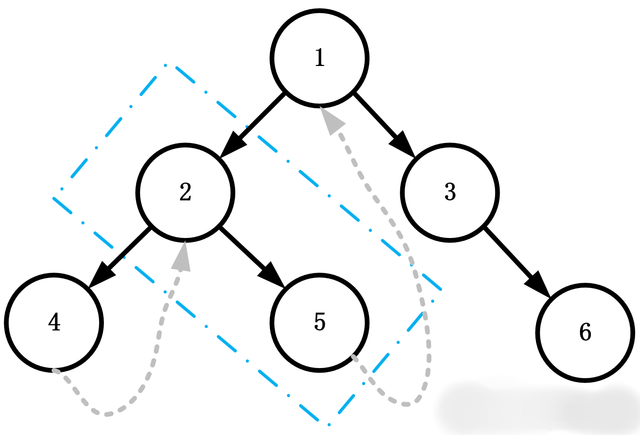
\includegraphics[scale=0.40]{images/morrisTraverse.png}
			%\caption{网页整体框架举例}
			\label{morrisTraverse}
		\end{center}
	\end{figure}
	\item 后序遍历PostOrderTraverse(T,Visit)):\\后序遍历的顺序是(左-->右-->根)。后序遍历采用的是简单的递归实现法,首先调用函数自身递归遍历其左子树,接着递归调用函数自身遍历其右子树,最后对当前结点调用visit()函数进行访问。特别注意,递归结束的条件是当前结点为空,因此需要在函数的入口处对当前结点是否为空进行判断,若为空,则应该使用return语句结束递归。
 	\item 按层遍历LevelOrderTraverse(T,Visit)):\\层序遍历的顺序是一层一层的遍历,即从左到右遍历完当前层后进入下一层。采用队列的方式进行层序遍历。我们将二叉树结点按层依次加入到队列中,并且保证在每一次循环开始时队列中的元素都来自同一层,接着对队列求长度,得到的长度就是当前层的结点个数。接着依次弹出这些结点,对于每一个结点,若该结点有左子树或右子树则将其加入到对立中,作为下一层的结点。开始循环之前我们将根结点加入到队列中作为第一层,当队列内为空时退出循环。
  	\item 增加二叉树addBinaryTree(forest, name, definition):\\首先判断森林是否已经满了,如果是,则直接返回ERROR。如果森林中还有空间,则声明一个根结点T,调用CreateBiTree()函数进行二叉树的创建,接着在森林中创建一个名字为name的二叉树并将其根结点赋值为T,最后让森林的大小增加1即可。
   	\item 最大路径和MaxPathSum(T):\\该函数的实现需要借助深度优先搜索的方式实现,因此需要定义一个辅助函数dfs(T, ans, nowSum)来实现,其中ans是用于返回结果的变量,应该初始化为一个很小的数(-0x3f3f3f3f),nowSum是当前得到的路径和。当dfs函数搜索到空结点时说明当前路径的搜索已经结束,若nowSum的值大于ans的值,则说明找到了一条新的路径使路径和更大,此时将ans的值更新为nowSum即可。在MaxPathSum()函数中我们先判断T是否为空,若是,则直接返回INFEASIBLE表示不可执行,若不为空,则分别对其左右子树调用dfs函数来,调用完成后即可将ans返回。
    \item 最近公共祖先LowestCommonAncestor(T,e1,e2):\\该函数的实现采用递归和回溯的方式实现,因此需要用到一个递归辅助函数isAncestor(T, a, b, ans)来判断T是否是a或者b的祖先(是则返回true,否则返回false),特别的,如果T是a或者b,也返回true。在递归函数isAncestor中首先判断当前结点T是否为空,若是,则直接返回false;若不是,则分别对T的左右子树调用isAncestor()函数判断T的左右子树是否为a或者b的祖先,若T的左右子树都是a或则b的祖先,或者其中一个子树为a或b的祖先且T为a或b,则说明T一定就是a与b的最小公共祖先,此时将ans赋值为T即可。在LowestCommonAncestor()函数中首先判断根结点是否为空,若为空,则直接返回NULL;若不为空则将ans初始化为NULL,接着对根结点调用一次isAncestor()函数即可得到ans,没有找到相应的结点,则ans将保留其初始值NULL不变。
    \item 翻转二叉树InvertTree(T):\\该函数的实现相对简单。需用用到一个递归辅助函数dfsInvert(T)来进行递归翻转。那为什么笔者不直接将InvertTree()写成递归的形式呢?这是因为在该函数中当根结点T为空时要返回INFEASIBLE(不可执行),而在递归中结束的标志是当前结点为空,递归结束时不需要返回任何值,故应该增加一个返回值为void的辅助函数完成递归。在dfsInvert()函数中笔者采用自底向上的翻转方式,首先递归的翻转当前结点T的左右子树,接则将T的左子树和右子树进行调换即可。在InvertTree()函数中我们先判断T是否为空,若为空,则返回INFEASIBLE,若不为空,则调用dfsInvert()函数进行翻转。
    \item 保存二叉树SaveBiTree(T, fileName):\\该函数仍需要一个辅助函数save(index, T, fp)来实现,其中index是当前结点T在满二叉树中的编号,fp是要写入的文件的指针(filePointor)。在save函数里,首先将当前结点的数据保存在一个unit类的对象p中,接着将对象p写入到文件中,再递归的保存其左子树和右子树,同时根据结点在满二叉树中的编号,index在进入左子树和右子树时分别变为index*2以及index*2+1。在SaveBiTree()函数中,首先判断根结点T是否为空,若是则直接返回OK表示空树不用存储,接着将文件指针初始化后调用save()函数进行保存,保存完成后将文件关闭即可。注意,在打开文件指针时应该判断打开是否成功,不成功则应该直接返回ERROR。
    \item 从文件中加载二叉树LoadBiTree(T, FileName):\\该函数首先判断T是否为空, 不为空则不能够将二叉树加载到其中,接着将文件指针初始化,将文件中的结点数据依次读出来保存在一个临时指针数组p中,以数组p的下标代表二叉树结点在满二叉树中的编号,根据父子编号的关系(父结点编号为n, 左孩子编号为n*2,右孩子编号为n*2+1),在相应的结点之间建立父子关系。在读取数据完成后将T赋值为p[1](根结点的编号为1)即可返回。注意,在打开文件指针时应该判断打开是否成功,若不成功则应该直接返回ERROR。
\end{enumerate}

%%%%%%%%%%%%%%%%%%%%%%%%%%%%%%%%%%%%%%%%%%%%%%%%%%%%%%%%%%%%%%%%%%%%%%%%%%%%%%
%%%%%%%%%%%%%%%%%%%%%%%%last here%%%%%%%%%%%%%%%%%%%%%%%%%%%%%%%%%%%%%%%%%%%%%

\subsection{系统测试}

主要说明针对各个函数正常和异常的测试用例及测试结果画图说明网页的整体框架,进行简要的文字描述等。画图说明网页的整体框架,进行简要的文字描述等。画图说明网页的整体框架,进行简要的文字描述等。画图说明网页的整体框架,进行简要的文字描述等。画图说明网页的整体框架,进行简要的文字描述等。画图说明网页的整体框架,进行简要的文字描述等。画图说明网页的整体框架,进行简要的文字描述等。

\subsection{实验小结}
\newpage




\section{课程的收获和建议}

描述通过学习该专题,有何收获,有何建议,如某专题可适当减少讲授时间、某专题可适当增加讲授内容和时间等。描述通过学习该专题,有何收获,有何建议,如某专题可适当减少讲授时间、某专题可适当增加讲授内容和时间等。描述通过学习该专题,有何收获,有何建议,如某专题可适当减少讲授时间、某专题可适当增加讲授内容和时间等。描述通过学习该专题,有何收获,有何建议,如某专题可适当减少讲授时间、某专题可适当增加讲授内容和时间等。

\subsection{基于顺序存储结构的线性表实现}

描述通过学习计算机基础知识专题,有何收获,有何建议,如某专题可适当减少讲授时间、某专题可适当增加讲授内容和时间等。描述网页的设计和实现过程中遇到的问题及如何解决。描述网页的设计和实现过程中遇到的问题及如何解决。描述网页的设计和实现过程中遇到的问题及如何解决。描述网页的设计和实现过程中遇到的问题及如何解决。描述网页的设计和实现过程中遇到的问题及如何解决。描述网页的设计和实现过程中遇到的问题及如何解决。描述网页的设计和实现过程中遇到的问题及如何解决。描述网页的设计和实现过程中遇到的问题及如何解决。

\subsection{基于链式存储结构的线性表实现}

描述通过学习文档撰写工具LaTeX专题,有何收获,有何建议,如某专题可适当减少讲授时间、某专题可适当增加讲授内容和时间等。描述通过学习文档撰写工具LaTeX专题,有何收获,有何建议,如某专题可适当减少讲授时间、某专题可适当增加讲授内容和时间等。

\subsection{基于二叉链表的二叉树实现}

描述通过学习编程工具Python专题,有何收获,有何建议,如某专题可适当减少讲授时间、某专题可适当增加讲授内容和时间等。描述通过学习编程工具Python专题,有何收获,有何建议,如某专题可适当减少讲授时间、某专题可适当增加讲授内容和时间等。

\subsection{基于二叉链表的二叉树实现}

描述通过学习计算机基础知识专题,有何收获,有何建议,如某专题可适当减少讲授时间、某专题可适当增加讲授内容和时间等。描述通过学习计算机基础知识专题,有何收获,有何建议,如某专题可适当减少讲授时间、某专题可适当增加讲授内容和时间等。


\nocite{*} %% 作用是不对文献进行引用,但可以生成文献列表

\bibliographystyle{Experimental_Report}
\bibliography{Experimental_Report}
\setcounter{secnumdepth}{0}
\appendix


\section{附录A 基于顺序存储结构线性表实现的源程序}

\noindent
/* Linear Table On Sequence Structure */\\
\#include <stdio.h>\\
\#include <malloc.h>\\
\#include <stdlib.h>\\

\noindent
/*---------page 10 on textbook ---------*/\\
\#define TRUE 1\\
\#define FALSE 0\\
\#define OK 1\\
\#define ERROR 0\\
\#define INFEASTABLE -1\\
\#define OVERFLOW -2\\
\newpage

\section{附录B 基于链式存储结构线性表实现的源程序}



\noindent

\begin{lstlisting}[title = Definition.h]
# ifndef DEFINITION_H_           // 防止头文件重复引入
# define DEFINITION_H_

#define TRUE 1                   // 状态宏定义 
#define FALSE 0
#define OK 1
#define ERROR 0
#define INFEASIBLE -1
#define OVERFLOW -2

#include <stdio.h>

typedef int status;
typedef int ElemType;            //数据元素类型定义

#define LIST_INIT_SIZE 100       // 初始大小以及增量的宏定义
#define LISTINCREMENT  10

typedef struct LNode{            //单链表(链式结构)结点的定义
	  ElemType data;
	  struct LNode *next;
	}LNode,*LinkList;            //单链表(链式结构)结点的定义

# endif	
\end{lstlisting}

\noindent

\begin{lstlisting}[title = Main.cpp]
# include <stdio.h>
# include "Definition.h"
# include "Init.h"
# include "Destroy.h"
# include "LocateElem.h"
# include "NextElem.h"
# include "PriorElem.h"
# include "ListInsert.h"
# include "ListTraverse.h"
# include "reverseList.h"
# include "RemoveNthFromEnd.h"
# include "sortList.h"
# include "saveandload.h"
# include "Clear.h"
# include "ListEmpty.h"
# include "GetElem.h"
# include "Lists.h"
# include "ListDelete.h"
# include "ListLength.h"

void showMenu(){
printf("========================================MENU===================================================\n"
"0 : Show this menu\n"
"1 : Initialize your list                     2 : Destroy your list\n"
"3 : Clear your list                          4 : Make sure if your list is empty\n"
"5 : Get the length of your lists             6 : Get one particular element\n"
"7 : Find the index of a particular element   8 : Get the prior of one element\n"
"9 : Get the next of one element              10: Insert element\n"
"11: Delete element                           12: Traverse your list\n"
"13: Reverse your list                        14: Delete one element from the end of your list\n"
"15: Sort your list                           16: Save your list in the file\n"
"17: Load your list from a file               18: Add some elements to your list\n"
"19: Choose a new list to operate             20: Quit\n"
"========================================MENU===================================================\n"
"\n");
}

int main(){
int tmp;
	
int choice, e, i, index, pre, next;
Lists lists;
// LinkList L = NULL;
int nowIndex = 0;
initLists(lists);

printf("choose a list from the lists! input an integer ranging from 1 to 20 : \n");
scanf("%d", &nowIndex);
printf("you chose list %d!\n", nowIndex);
putchar('\n');

LinkList tmpl = NULL, tailOftmpl;
status sta;
char f[100];

	
showMenu();
printf("MAKE YOUR CHOICE!\n");
while(true){
scanf("%d", &choice);
switch(choice){
case 0:
	showMenu();
	break;
case 1:
	sta = InitList(lists.list[nowIndex]);
	lists.listTail[nowIndex] = lists.list[nowIndex];
	if (sta == OK){
		printf("OK!\n");
	}else{
		printf("this list can not be initialized!\n");
	}
	break;
case 2:
if (lists.list[nowIndex] == NULL){
		printf("this list hasn't been initialized!\n");
		break;
	}
	sta = DestroyList(lists.list[nowIndex]);
	if (sta == OK){
		printf("OK!\n");
	}else{
		printf("this list can not be Destroyed!\n");
	}
	break;
case 3:
	if (lists.list[nowIndex] == NULL){
		printf("this list hasn't been initialized!\n");
		break;
	}
	sta = ClearList(lists.list[nowIndex]);
	if (sta == OK){
		printf("OK!\n");
	}else{
		printf("this list can not be cleared!\n");
	}
	break;
case 4:
	sta = ListEmpty(lists.list[nowIndex]);
	if (sta == INFEASIBLE){
		printf("this list does not exist!\n");
	}else if (sta == true){
		printf("this list is empty!\n");
	}else{
		printf("this list is not empty!\n");
	}
	break;
case 5:
	sta = ListLength(lists.list[nowIndex]);
	if (sta == INFEASIBLE){
		printf("this list does not exist!\n");
	}else{
		printf("this list's length = %d!\n", sta);
	}
	break;
case 6:
	printf("input the index of the element in the list!\n");
	scanf("%d", &index);
	sta = GetElem(lists.list[nowIndex],index,e);
	if (sta == INFEASIBLE){
		printf("this list does not exist!\n");
	}else if (sta ==ERROR){
		printf("this index does not exist in the list!\n");
	}else{
		printf("you get it : %d!\n", e);
	}
	break;
case 7:
	printf("input the element you want to find in the list!\n");
	scanf("%d", &e);
	sta = LocateElem(lists.list[nowIndex],e);
	if (sta == INFEASIBLE){
		printf("this list does not exist!\n");
	}else if (sta ==ERROR){
		printf("this element does not exist in the list!\n");
	}else{
		printf("you get its index : %d!\n", sta);
	}
	break;
case 8:
	printf("input the element whose prior element you want to find in the list!\n");
	scanf("%d", &e);
	sta = PriorElem(lists.list[nowIndex],e,pre);
	if (sta == INFEASIBLE){
		printf("this list does not exist!\n");
	}else if (sta ==ERROR){
		printf("this prior does not exist in the list!\n");
	}else{
		printf("you get its prior one : %d!\n", pre);
	}
	break;
case 9:
	printf("input the element whose next element you want to find in the list!\n");
	scanf("%d", &e);
	sta = NextElem(lists.list[nowIndex],e,next);
	if (sta == INFEASIBLE){
		printf("this list does not exist!\n");
	}else if (sta ==ERROR){
		printf("this next does not exist in the list!\n");
	}else{
		printf("you get its next one : %d!\n", next);
	}
	break;
case 10:
	if (lists.list[nowIndex] == NULL){
		printf("this list hasn't been initialized!\n");
		break;
	}
	printf("input the element you want to insert in the list!\n");
	scanf("%d", &e);
	printf("input the index you want to insert in the list!\n");
	int index;
	scanf("%d", &index);
	sta = ListInsert(lists.list[nowIndex],index,e);
	if (sta == INFEASIBLE){
		printf("this list does not exist!\n");
	}else if (sta ==ERROR){
		printf("this index does not exist in the list!\n");
	}else{
		printf("OK!\n");
	}
	break;
case 11:
	if (lists.list[nowIndex] == NULL){
		printf("this list hasn't been initialized!\n");
		break;
	}
	printf("input the index you want to delete in the list!\n");
	scanf("%d", &index);
	sta = ListDelete(lists.list[nowIndex],index,e);
	if (sta == INFEASIBLE){
		printf("this list does not exist!\n");
	}else if (sta ==ERROR){
		printf("this index does not exist in the list!\n");
	}else{
		printf("you have deleted %d\n", e);
	}
	break;
case 12:
	sta = ListTraverse(lists.list[nowIndex]);
	if (sta == INFEASIBLE){
		printf("this list does not exist!\n");
	}else{
		printf("OK!\n");
	}
	break;
case 13:
	sta = reverseList(lists.list[nowIndex]);
	if (sta == INFEASIBLE){
		printf("this list does not exist!\n");
	}else{
		printf("OK!\n");
	}
	break;
case 14:
	if (lists.list[nowIndex] == NULL){
		printf("this list hasn't been initialized!\n");
		break;
	}
	printf("input the index (from the bottom) you want to delete in the list!\n");
	scanf("%d", &index);
	sta = RemoveNthFromEnd(lists.list[nowIndex],index, e);
	if (sta == INFEASIBLE){
		printf("this list does not exist!\n");
	}else if (sta ==ERROR){
		printf("this index does not exist in the list!\n");
	}else{
		printf("you have deleted %d\n", e);
	}
	break;
case 15:
	sta = sortList(lists.list[nowIndex]);
	if (sta == INFEASIBLE){
		printf("this list does not exist!\n");
	}else{
		printf("OK!\n");
	}
	break;
case 16:
	printf("input the filename where you want to save the list!\n");
	scanf("%s", f);
	sta = SaveList(lists.list[nowIndex], f);
	if (sta == INFEASIBLE){
		printf("this list does not exist!\n");
	}else if (sta == ERROR){
		printf("open error!\n");
	}else{
		printf("OK!\n");
	}
	break;
case 17:
	printf("input the filename where you want to load the list!\n");
	scanf("%s", f);
	sta = LoadList(lists.list[nowIndex], f);
	if (sta == INFEASIBLE){
		printf("this list isn't empty so you can't load anything onto it!\n");
	}else if (sta == ERROR){
		printf("open error!\n");
	}else{
		printf("OK!\n");
	}
	break;
case 18:                            //添加一串元素;	
if (lists.list[nowIndex] == NULL){
	printf("this list hasn't been initialized!\n");
	break;
}
	printf("input a list ended with 0!\n");
	
	tmpl = (LinkList)malloc(sizeof(LNode));
	tailOftmpl = tmpl;
	scanf("%d", &tmp);
	while(tmp != 0){
		LinkList p = (LinkList)malloc(sizeof(LNode));
		p->data = tmp;
		tailOftmpl->next = p;
		tailOftmpl = p;
		scanf("%d", &tmp);
	}
	tailOftmpl->next = NULL;
	lists.listTail[nowIndex]->next = tmpl->next;
	lists.listTail[nowIndex] = tailOftmpl;
	free(tmpl);
	printf("OK!\n");
	break;
case 19:
	printf("choose a list from the lists! input an integer ranging from 1 to 20 : \n");
	scanf("%d", &nowIndex);
	printf("you chose list %d!\n", nowIndex);
	break;
case 20:
	goto out;
		}     
	}
	out :
	return 0;
}	
\end{lstlisting}

\begin{lstlisting}[title = Init.h]
# ifndef INIT_H_                // 防止头文件重复引入
# define INIT_H_
# include "Definition.h"
# include <malloc.h>
status InitList(LinkList&);   // 函数声明
# endif
\end{lstlisting}

\begin{lstlisting}[title = Init.cpp]
# include "Init.h"
status InitList(LinkList &L)
{
    if (L != NULL)                            // 若L已经非空,则不能初始化
        return INFEASIBLE;
    L = (LinkList)malloc(sizeof(LNode));     // 创建结点
    L->next = NULL;                          // 结点的下一结点设为空
    return OK;
}
\end{lstlisting}

\begin{lstlisting}[title = Destroy.h]
# ifndef DESTROY_H_                // 防止头文件重复引入
# define DESTROY_H_
# include "Definition.h"
# include <malloc.h>
status DestroyList(LinkList &);   // 函数声明
# endif
\end{lstlisting}

\begin{lstlisting}[title = Destroy.cpp]
# include "Destroy.h"
status DestroyList(LinkList &L)
{

    if (L == NULL)                              // 表是空的不能销毁
        return INFEASIBLE;
    LinkList p = L->next;                       // 从第一个元素开始销毁
    while (p != NULL){
        LinkList tmp = p->next;
        free(p);
        p = tmp;
    }
    free(L);                                    // 将表结点销毁后设置为空
    L = NULL;
    return OK;
}
\end{lstlisting}

\begin{lstlisting}[title = Clear.h]
# ifndef CLEAR_H_               // 防止头文件重复引入
# define CLEAR_H_
# include "Definition.h"
# include <malloc.h>
status ClearList(LinkList&);   // 初始化链表的函数声明
# endif
\end{lstlisting}

\begin{lstlisting}[title = Clear.cpp]
# include "Clear.h"
status ClearList(LinkList &L)
{
    if (L == NULL)                          // 表不存在不能清空!
        return INFEASIBLE;   
    LinkList p = L->next;                   // 将从表的第一个元素开始清空!
    while (p){
        LinkList tmp = p->next;
        free(p);
        p = tmp;
    }
    L->next = NULL;                         //  清空操作不能删除表头结点!
    return OK;
}
\end{lstlisting}

\begin{lstlisting}[title = ListEmpty.h]
# ifndef LISTEMPTY_H_                // 防止头文件重复引入
# define LISTEMPTY_H_
# include "Definition.h"
status ListEmpty(LinkList);   // 函数声明
# endif
\end{lstlisting}

\begin{lstlisting}[title = ListEmpty.cpp]
# include "ListEmpty.h"
status ListEmpty(LinkList L)
{
    if (L == NULL)                          // 表不存在,不能判断!
        return INFEASIBLE;
    return L->next == NULL;                 // 表是空的意味着结点的下一结点是空!
}
\end{lstlisting}

\begin{lstlisting}[title = ListLength.h]
# ifndef LISTLENGTH_H_                // 防止头文件重复引入
# define LISTLENGTH_H_
# include "Definition.h"
# include <malloc.h>
int ListLength(LinkList);   // 函数声明
# endif
\end{lstlisting}

\begin{lstlisting}[title = ListLength.cpp]
# include "ListLength.h"
int ListLength(LinkList L)
{
    if (L == NULL)                              // 表不存在,不能读取长度!
        return INFEASIBLE;
    int cnt = 0;
    LinkList p = L->next;                       // 从第一个元素开始算!
    while (p){
        cnt ++;
        p = p->next;
    }
    return cnt;                                 // 返回结果!
}
\end{lstlisting}

\begin{lstlisting}[title = GetElem.h]
# ifndef GETELEM_H_                // 防止头文件重复引入
# define GETELEM_H_
# include "Definition.h"
# include "ListLength.h"
status GetElem(LinkList, int, ElemType&);   // 函数声明
# endif
\end{lstlisting}

\begin{lstlisting}[title = GetElem.cpp]
# include "GetElem.h"
status GetElem(LinkList L,int i,ElemType &e)
{
    if (L == NULL)
        return INFEASIBLE;
    int length = ListLength(L);
    if (i < 1 || i > length)
        return ERROR;
    LinkList p = L;
    while (i--){
        p = p->next;
    }
    e = p->data;
    return OK;
}
\end{lstlisting}

\begin{lstlisting}[title = LocateElem.h]
# ifndef LOCATEELEM_H_                // 防止头文件重复引入
# define LOCATEELEM_H_
# include "Definition.h"
status LocateElem(LinkList L,ElemType e);   // 函数声明
# endif
\end{lstlisting}

\begin{lstlisting}[title = LocateElem.cpp]
# include "LocateElem.h"
status LocateElem(LinkList L,ElemType e)
{
    if (L == NULL)
        return INFEASIBLE;
    LinkList p = L->next;
    int index = 1;
    while (p){
        if (p->data == e)
            return index;
        index ++;
        p = p->next;
    }
    return ERROR;
}
\end{lstlisting}

\begin{lstlisting}[title = PriorElem.h]
# ifndef PIRORELEM_H_                // 防止头文件重复引入
# define PIRORELEM_H_
# include "Definition.h"
status PriorElem(LinkList ,ElemType,ElemType& );   // 函数声明
# endif
\end{lstlisting}

\begin{lstlisting}[title = PriorElem.cpp]
# include "PriorElem.h"
status PriorElem(LinkList L,ElemType e,ElemType &pre)
{
    if (L == NULL)
        return INFEASIBLE;
    LinkList p = L->next;
    while (p && p->next){
        if (p->next->data == e){
            pre = p->data;
            return OK;
        }
        p = p->next;
    }
    return ERROR;
}
\end{lstlisting}

\begin{lstlisting}[title = NextElem.h]
# ifndef NEXTELEM_H_                // 防止头文件重复引入
# define NEXTELEM_H_
# include "Definition.h"
status NextElem(LinkList ,ElemType ,ElemType& );   // 函数声明
# endif
\end{lstlisting}

\begin{lstlisting}[title = NextElem.cpp]
# include "NextElem.h"

status NextElem(LinkList L,ElemType e,ElemType &next)
{
    if (L == NULL)
        return INFEASIBLE;

    LinkList p = L->next;
    while (p && p->next){
        if (p->data == e){
            next = p->next->data;
            return OK;
        }
        p = p->next;
    }
    
    return ERROR;

}
\end{lstlisting}

\begin{lstlisting}[title = ListInsert.h]
# ifndef LISTINSERT_H_                // 防止头文件重复引入
# define LISTINSERT_H_

# include "Definition.h"
# include <malloc.h>

status ListInsert(LinkList& ,int ,ElemType );   // 函数声明

# endif
\end{lstlisting}

\begin{lstlisting}[title = ListInsert.cpp]
# include "ListInsert.h"

status ListInsert(LinkList &L,int i,ElemType e)
{
    if (L == NULL)
        return INFEASIBLE;
    
    if (i < 1)
        return ERROR;

    int index = 1;
    LinkList p = L;
    while (p && index < i){
        p = p->next;
        index ++;
    }
    
    if (p == NULL)
        return ERROR;

    if (p->next == NULL){
        p->next = (LinkList)malloc(sizeof(LNode));
        p = p->next;
        p->data = e;
        p->next = NULL;
    }else{
        LinkList tmp = (LinkList)malloc(sizeof(LNode));
        tmp->data = e;
        tmp->next = p->next;
        p->next = tmp;
    }
    return OK;
}
\end{lstlisting}

\begin{lstlisting}[title = ListDelete.h]
# ifndef LISTDELETE_H_                // 防止头文件重复引入
# define LISTDELETE_H_
# include "Definition.h"
# include <malloc.h>
status ListDelete(LinkList&, int, ElemType& );   // 函数声明
# endif
\end{lstlisting}

\begin{lstlisting}[title = ListDelete.cpp]
# include "ListDelete.h"
status ListDelete(LinkList &L,int i,ElemType &e)
{
    if (L == NULL)
        return INFEASIBLE; 
    if (i < 1)
        return ERROR;
    int index = 1;
    LinkList p = L;
    while (p && index < i){
        p = p->next;
        index ++;
    }
    if (p == NULL || p->next == NULL)
        return ERROR;
    e = p->next->data;
    LinkList tmp = p->next;
    p->next = tmp->next;
    free(tmp); 
    return OK;
}

\end{lstlisting}

\begin{lstlisting}[title = ListTraverse.h]
# ifndef LISTTRAVERSE_H_                // 防止头文件重复引入
# define LISTTRAVERSE_H_

# include "Definition.h"
# include <stdio.h>

status ListTraverse(LinkList );   // 函数声明

# endif
\end{lstlisting}

\begin{lstlisting}[title = ListTraverse.cpp]
# include "ListTraverse.h"

status ListTraverse(LinkList L)
{
    if (L == NULL)
        return INFEASIBLE;

    LinkList p = L->next;

    while (p){
        printf("%d", p->data);
        // if (p->next != NULL)
            putchar(' ');
        p = p->next;
    }
    return OK;

}
\end{lstlisting}

\begin{lstlisting}[title = reverseList.h]
# ifndef REVERSELIST_H_                // 防止头文件重复引入
# define REVERSELIST_H_

# include "Definition.h"
# include "ListLength.h"

status reverseList(LinkList&);   // 函数声明

# endif
\end{lstlisting}

\begin{lstlisting}[title = reverseList.cpp]
# include "reverseList.h"

status reverseList(LinkList& L){
    if (L == NULL)
        return INFEASIBLE;

    if (L->next == NULL)
        return OK;

    LinkList p = L, tmp = p->next;

    while (p && tmp){
        LinkList tmpp = tmp->next;
        if (p != L)
            tmp->next = p;
        else
            tmp->next = NULL;
        p = tmp;
        tmp = tmpp;
    }

    L->next = p;
    
    return OK;
}
\end{lstlisting}

\begin{lstlisting}[title = RemoveNthFromEnd.h]
# ifndef REMOVENTHFROMEND_H_                // 防止头文件重复引入
# define REMOVENTHFROMEND_H_

# include "Definition.h"
# include "ListLength.h"
# include "ListDelete.h"

status RemoveNthFromEnd(LinkList&, int, int& );   // 函数声明

# endif
\end{lstlisting}

\begin{lstlisting}[title = RemoveNthFromEnd.cpp]
# include "RemoveNthFromEnd.h"

status RemoveNthFromEnd(LinkList& L, int n, int& e){
    if (L == NULL)
        return ERROR;
    
    int len = ListLength(L);
    n = len - n + 1;

    return ListDelete(L, n, e);
}
\end{lstlisting}

\begin{lstlisting}[title = sortList.h]
# ifndef SORTLIST_H_                // 防止头文件重复引入
# define SORTLIST_H_

# include "Definition.h"
# include "ListLength.h"

status sortList(LinkList);   // 函数声明
void quickSort(ElemType[], int, int);
# endif
\end{lstlisting}

\begin{lstlisting}[title = sortList.cpp]
# include "sortList.h"

void quickSort(ElemType arr[], int i, int j){
    if (i >= j)
        return;

    int low = i;
    int high = j;
    ElemType k = arr[low];
    
    while (low < high){
        while (low < high && k <= arr[high]){
            high --;
        }

        if (low < high && k > arr[high]){
            arr[low] = arr[high];
            low ++;
        }

        while (low < high && k >= arr[low]){
            low ++;
        }

        if (low < high && k < arr[low]){
            arr[high] = arr[low];
            high --;
        }
    }
    arr[low] = k;

    quickSort(arr, i, low-1);
    quickSort(arr, low+1, j);
}

status sortList(LinkList L){
    if (L == NULL)
        return INFEASIBLE;
    
    if (L ->next == NULL)
        return OK;

    int len = ListLength(L);
    ElemType arr[len];
    LinkList p = L->next;
    
    for (int i = 0; i < len; p = p->next, i++){
        arr[i] = p->data;
    }

    quickSort(arr, 0, len-1);

    p = L->next;

    for (int i = 0; i < len; p = p->next, i++){
        p->data = arr[i];
    }

    return OK;
}
\end{lstlisting}

\begin{lstlisting}[title = saveandload.h]
# ifndef SAVEANDLOAD_H_                // 防止头文件重复引入
# define SAVEANDLOAD_H_

# include "Definition.h"
# include <malloc.h>
# include <stdio.h>

status SaveList(LinkList ,char []);   // 函数声明
status LoadList(LinkList&, char []);

# endif
\end{lstlisting}

\begin{lstlisting}[title = saveandload.cpp]
# include "saveandload.h"

status SaveList(LinkList L,char FileName[])
{
    if (L == NULL)
        return INFEASIBLE;
    
    FILE* fp = NULL;
    fp = fopen(FileName, "wb");
    if (fp == NULL)
        return ERROR;
    
    LinkList p = L->next;
    while (p){
        fwrite(&p->data, sizeof(ElemType), 1, fp);
        p = p->next;
    }
    fclose(fp);

    return OK;

}

status LoadList(LinkList &L,char FileName[])
{
    if (L != NULL && L->next != NULL)
        return INFEASIBLE;
    
    FILE* fp = NULL;
    fp = fopen(FileName, "rb");
    if (fp == NULL)
        return ERROR;
    
    free(L);
    L = NULL;
    L = (LinkList)malloc(sizeof(LNode));
    LinkList tail = L;
    while (fgetc(fp) != EOF){
        fseek(fp, -1, SEEK_CUR);
        
        LinkList tmp = (LinkList)malloc(sizeof(LNode));
        fread(&tmp->data, sizeof(ElemType), 1, fp);
        tail->next = tmp;
        tail = tmp;
    }
    tail->next = NULL;
    fclose(fp);
    return OK;

}

\end{lstlisting}

\begin{lstlisting}[title = lists.h]
# ifndef LISTS_H_               // 防止头文件重复引入
# define LISTS_H_
# include "Definition.h"
# include "Destroy.h"
# include <malloc.h>
#define LISTS_INIT_SIZE 21
typedef struct {                 
      LinkList* list;
      LinkList* listTail;
      int length;
      int size;
}Lists;
status initLists(Lists&);
# endif

\end{lstlisting}

\begin{lstlisting}[title = lists.cpp]
# include "Lists.h"
status initLists(Lists& lists){
    lists.length = 0;
    lists.size = LISTS_INIT_SIZE;
    lists.list = NULL;
    lists.list = (LinkList*)malloc(sizeof(LinkList)*(LISTS_INIT_SIZE));
    if (lists.list == NULL){
        return ERROR;
    }
    lists.listTail = NULL;
    lists.listTail = (LinkList*)malloc(sizeof(LinkList)*(LISTS_INIT_SIZE));
    if (lists.listTail == NULL){
        return ERROR;
    }

    for (int i = 0; i < lists.size; i++){
        lists.list[i] = NULL;
        lists.listTail[i] = NULL;
    }

    return OK;
}
\end{lstlisting}









%\begin{lstlisting}[title = sortList.cpp]
%# ifndef CLEAR_H_               // 防止头文件重复引入
%# define CLEAR_H_
%
%# include "Definition.h"
%# include <malloc.h>
%
%status ClearList(LinkList&);   // 初始化链表的函数声明
%
%# endif
%\end{lstlisting}







\newpage



\section{附录C 基于二叉链表二叉树实现的源程序}
\newpage


\section{附录D 基于邻接表图实现的源程序}

\end{document}